\documentclass{beamer}
\usetheme{CambridgeUS}
%\usetheme{Boadilla}
\usecolortheme{beaver}
\usepackage{wrapfig}
\usepackage{amsmath}
\usepackage{kbordermatrix}
\usepackage[justification=centering]{caption}
\captionsetup[figure]{labelformat=empty}
\usepackage{tikz}
	
\setbeamertemplate{section in toc}{%
\leavevmode\leftskip=5.65ex%
  \llap{\raisebox{0.2ex}{\textcolor{darkred}{$\blacktriangleright$}}\kern1ex}%
  \inserttocsection\par%
}


%remove the icon
\setbeamertemplate{bibliography item}{}

%remove line breaks
\setbeamertemplate{bibliography entry title}{}
\setbeamertemplate{bibliography entry location}{}
\setbeamertemplate{bibliography entry note}{}

\makeatother
\setbeamertemplate{footline}
{
  \leavevmode%
  \hbox{%
  \begin{beamercolorbox}[wd=.3\paperwidth,ht=2.25ex,dp=1ex,center]{author in head/foot}%
    \usebeamerfont{author in head/foot}\insertshortauthor
  \end{beamercolorbox}%
  \begin{beamercolorbox}[wd=.7\paperwidth,ht=2.25ex,dp=1ex,center]{title in head/foot}%
    \usebeamerfont{title in head/foot}\insertshorttitle\hspace*{3em}
    \insertframenumber{} / \inserttotalframenumber\hspace*{1ex}
  \end{beamercolorbox}}%
  \vskip0pt%
}
\makeatletter
\setbeamertemplate{navigation symbols}{}
\setbeamertemplate{itemize items}[default]
\DeclareCaptionFont{tiny}{\tiny}

%\makeatother
%\theoremstyle{mystyle}
%\newtheorem*{environment}{Definition}

\makeatother
\theoremstyle{mystyle}
\newtheorem*{scenario}{Scenarios}

%***************************

\title{Learning Math - Whose Idea Was That?! }
\author{Jessica Sorrell}
\institute{EMC}
\date{June 29, 2016}

\begin{document}

%***************************

\begin{frame}
	\titlepage
\end{frame}

%***************************
\section*{Outline}

\begin{frame}
	\frametitle{Outline}
	\tableofcontents

\end{frame}

%***************************
\section{Introduction}
\frame{\tableofcontents[currentsection]}

\begin{frame}

\end{frame}

%***************************
\section{High School}
\frame{\tableofcontents[currentsection]}

\begin{frame}

\begin{center}
	
\includegraphics[scale=0.5]{desa.jpg}
	
	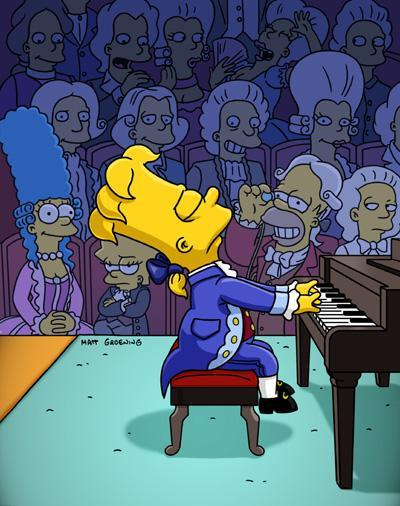
\includegraphics[scale=0.35]{bartpianist.jpg}
\end{center}

\end{frame}
%***************************


\begin{frame}
\frametitle{``What's wrong here?"}

\[\text{Let } x = 1\]

\pause

\[x = x^2\]

\pause

\[x - 1 = x^2 - 1\]

\pause

\[\frac{x - 1}{x - 1} = \frac{x^2 - 1}{x - 1}\]

\pause

\[ 1 = x+1\]

\pause

\[1 = 2\]
\end{frame}

%***************************

\begin{frame}
\frametitle{Mr. Johnson's Classroom }

\vspace{0.1in}
\begin{columns}
	\begin{column}{0.48\textwidth}
		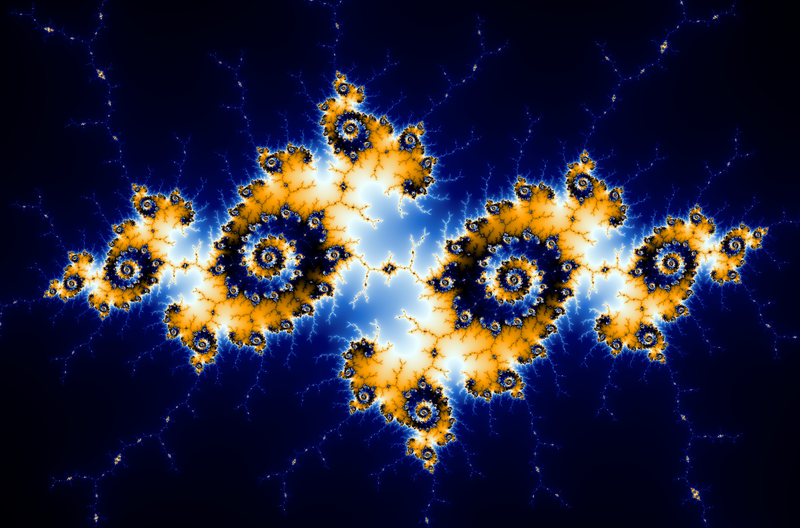
\includegraphics[scale=0.19]{mandelbrot.png}
	\end{column}
	\begin{column}{0.48\textwidth}
		\includegraphics[scale=0.11]{mandelbrot2.jpeg}
	\end{column}
\end{columns}

\begin{center}
	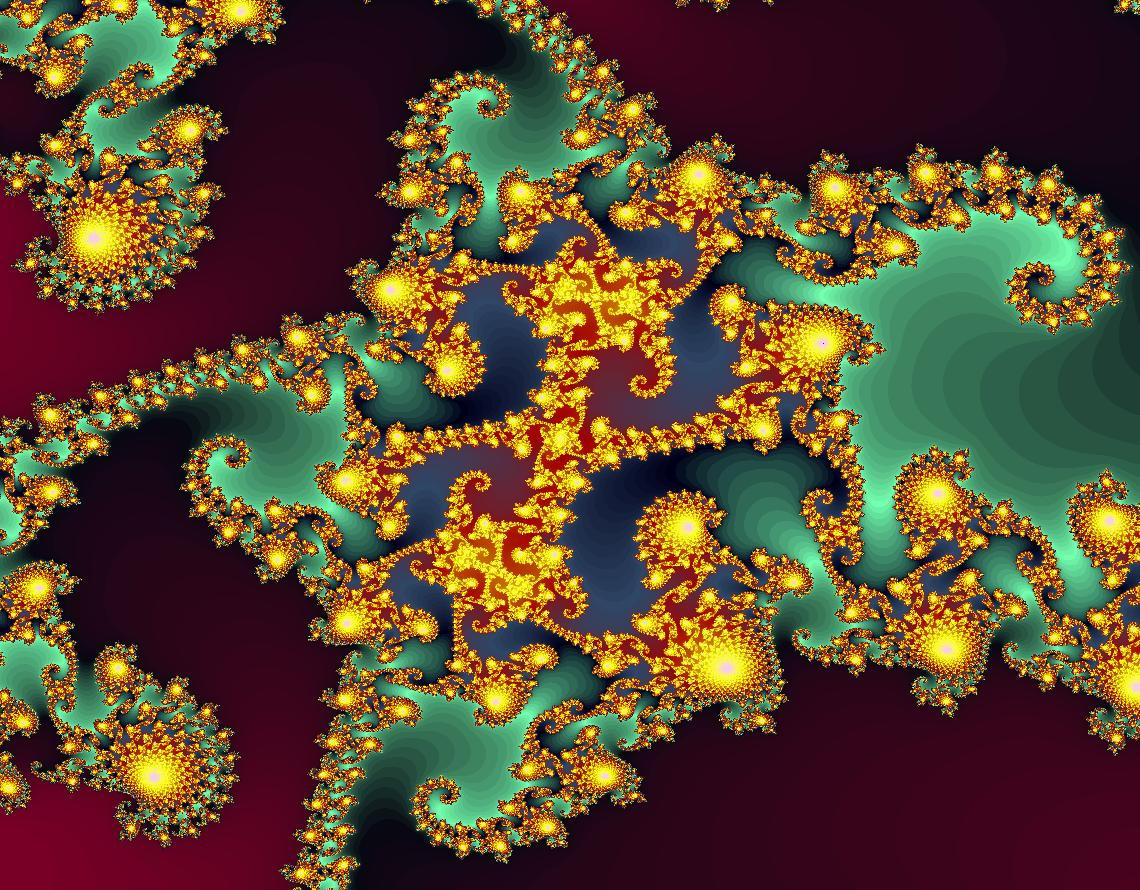
\includegraphics[scale=0.11]{fractal1.jpg}
\end{center}
\end{frame}

%***************************

\begin{frame}
\frametitle{...Is Mr. Johnson a Tool fan?}

\begin{center}
	\begin{figure}
		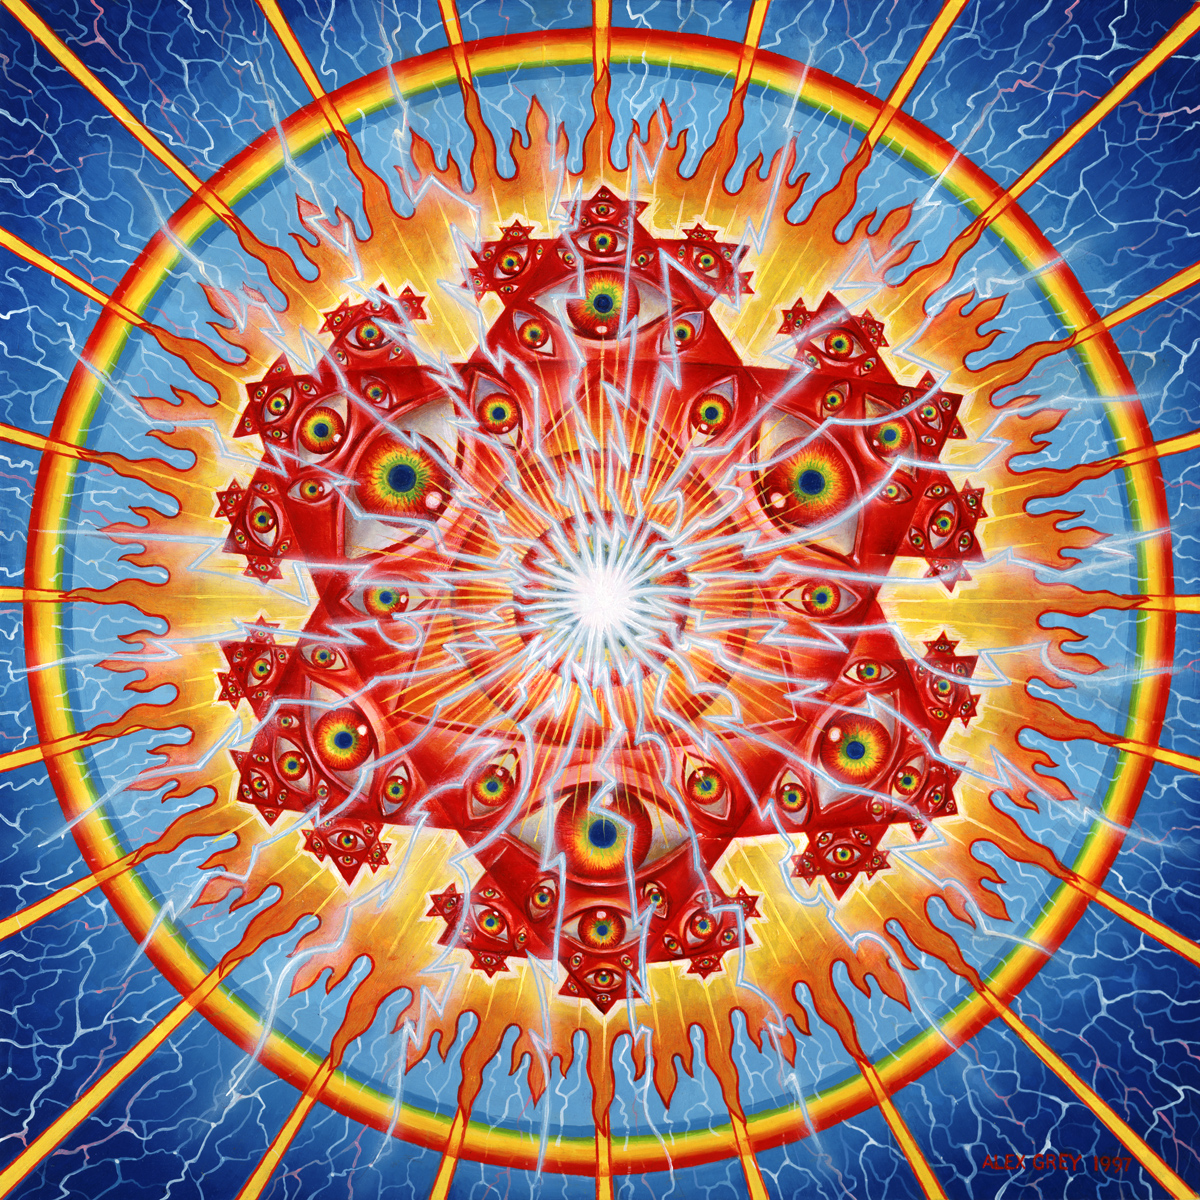
\includegraphics[scale=0.15]{lateralus.jpg}
		\caption{Vision Crystal by Alex Grey}
	\end{figure}
\end{center}

\end{frame}
%***************************

\begin{frame}
\frametitle{Fractals}

\begin{center}
"The Mandelbrot set is the set of complex numbers $c$ for which the function
\[ f_c(z) = z^2 + c\]
does not diverge when iterated from $z = 0$ ..."
\end{center} 
\hspace{3in}- Wikipedia

\pause 

\begin{center}
	
\includegraphics[scale=0.3]{bart}
\end{center}

\end{frame}
%***************************

\begin{frame}
\frametitle{What Mr. Johnson Taught Me}

\begin{columns}
	\column{0.6\textwidth}
		Math is not an arbitrary set of rules created by the ur-teacher\\
	\column{0.35\textwidth}
		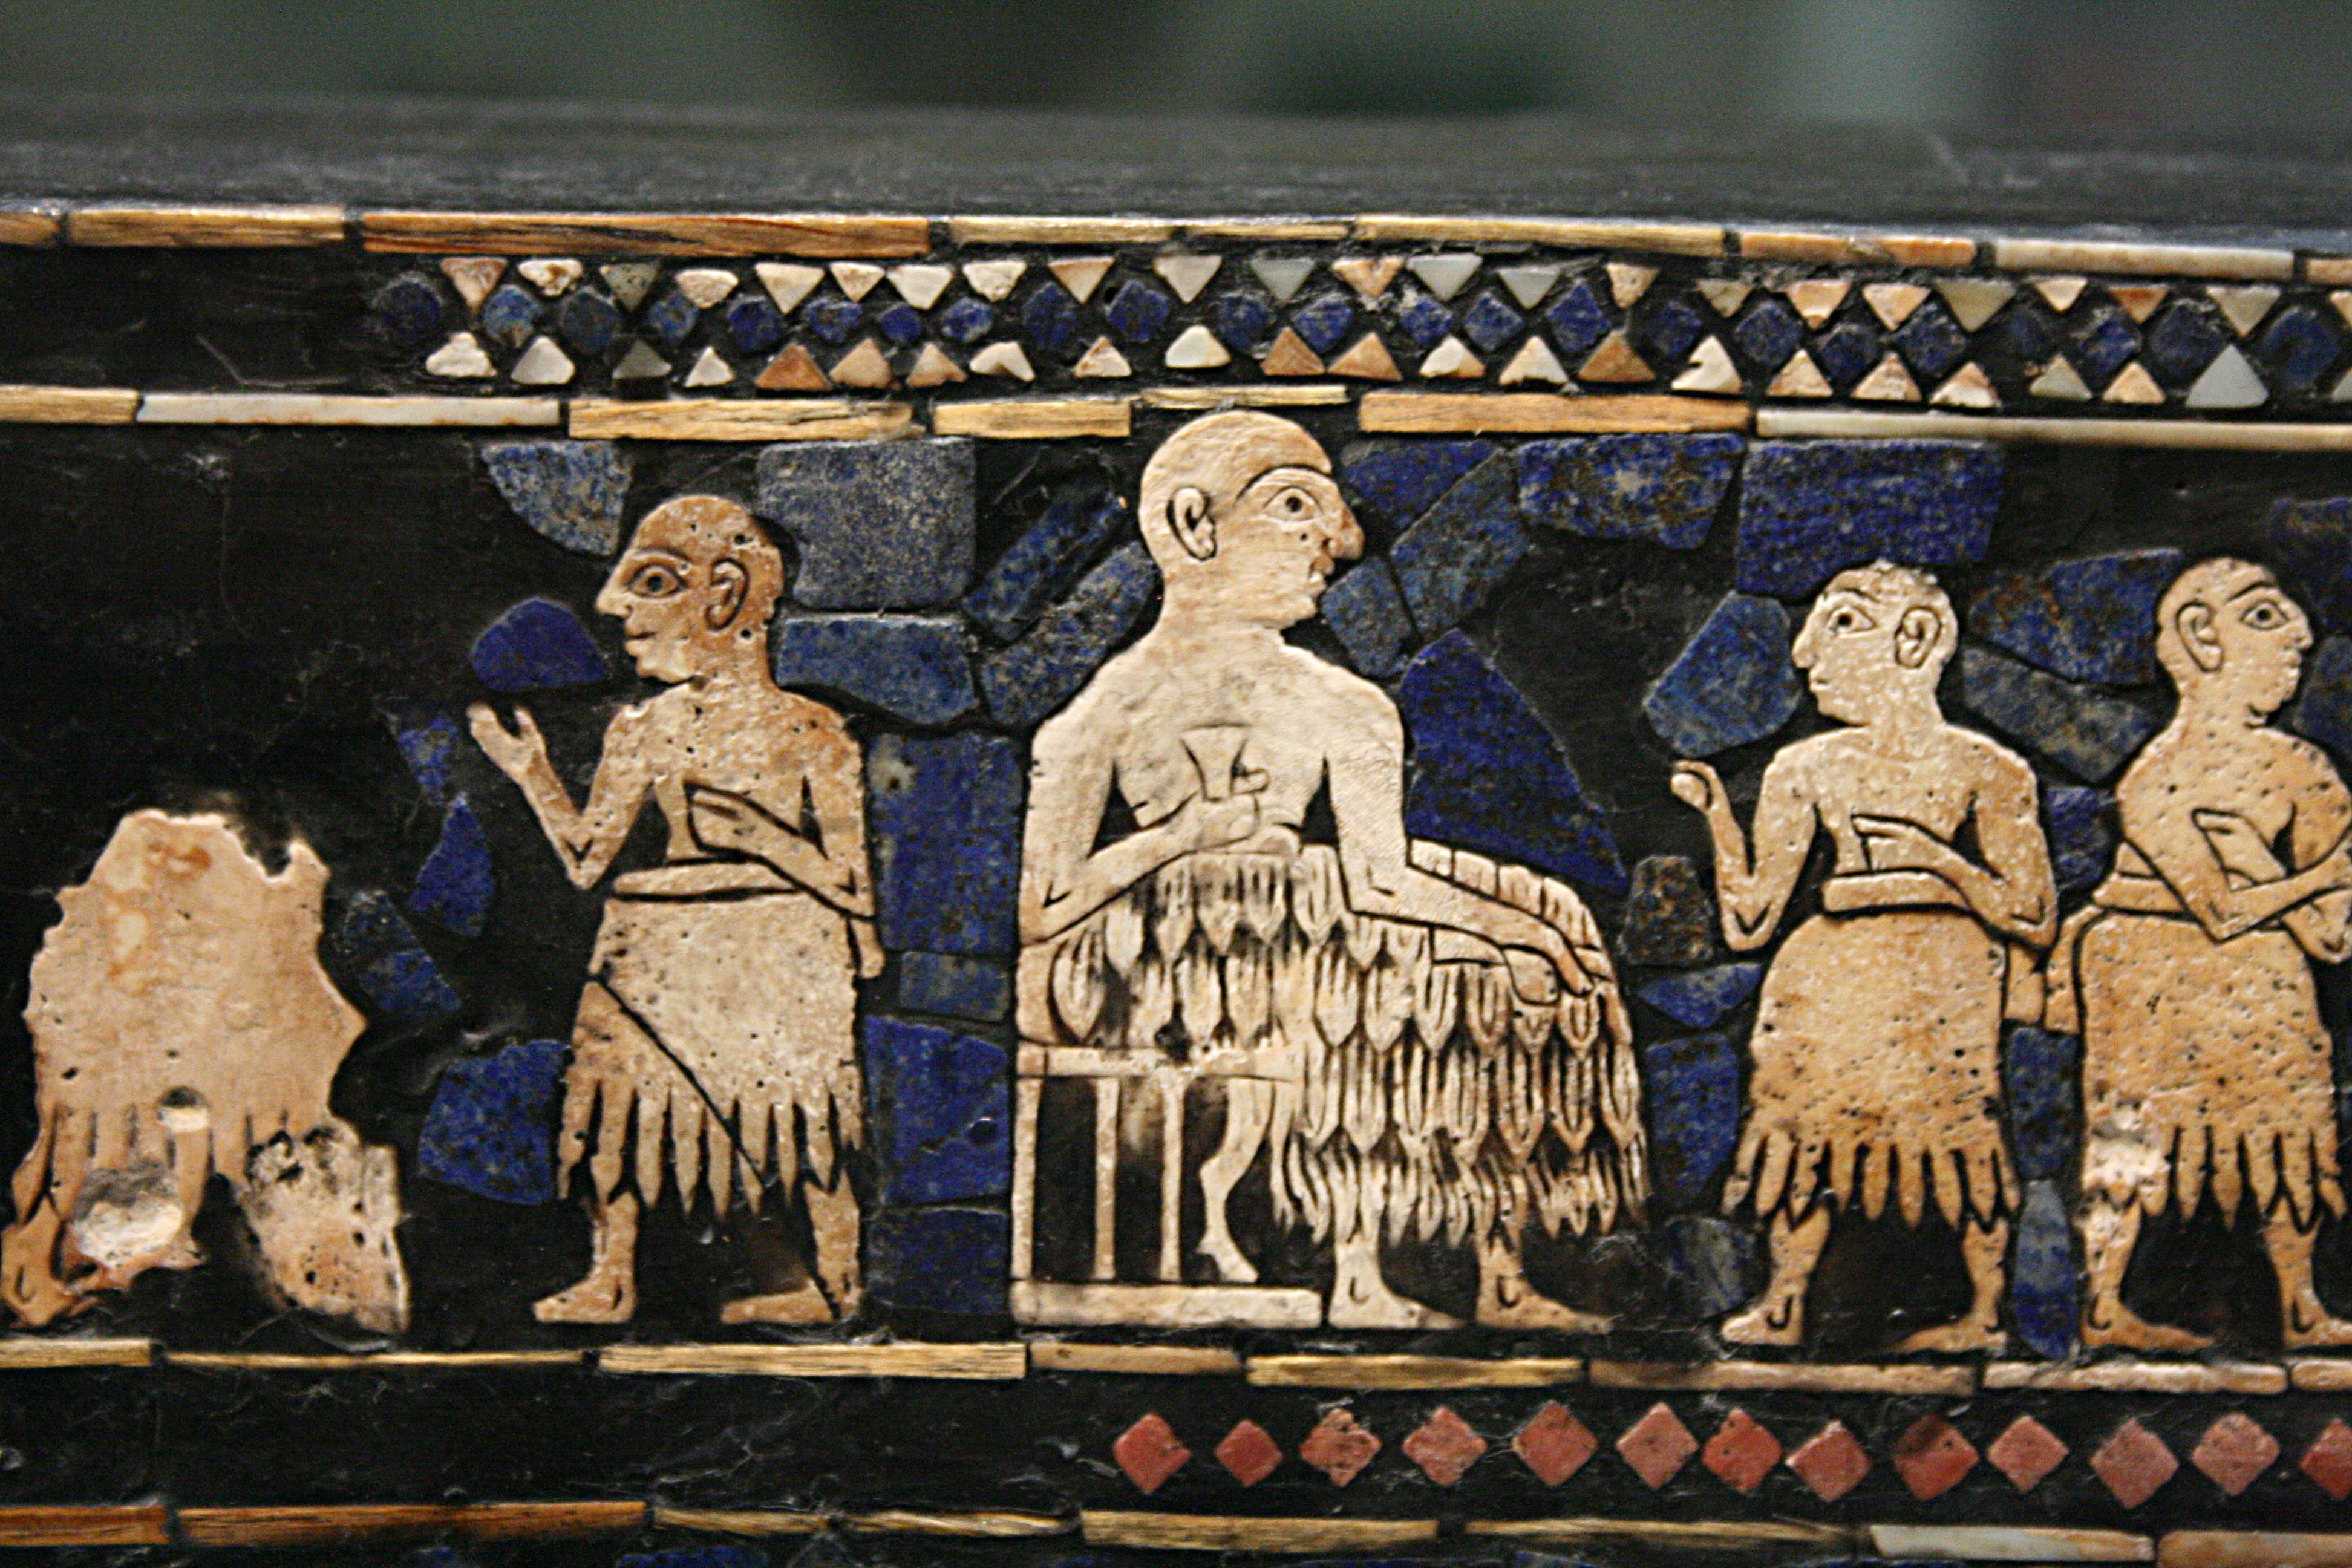
\includegraphics[scale=0.027]{ur.jpg}
\end{columns} 
	\pause
\begin{columns}
	\column{0.35\textwidth}	
		\includegraphics[scale=0.022]{/home/hatgirl/dev/algoart/barbedwire/barbed_wire}		
	\column{0.55\textwidth}
		Simple rules can yield complex structure
\end{columns}
	\pause
\begin{columns}
	\column{0.14\textwidth}	
		Calculus!
	\column{0.65\textwidth}
		\[f(a) + \frac{f'(a)}{1!}(x-a) + \frac{f''(a)}{2!}(x-a)^2 + \frac{f''(a)}{3!}(x-a)^3 + ... \]		
\end{columns}

\end{frame}

%***************************
\begin{frame}
\frametitle{What Mr. Johnson Taught Me}
	Math is a set of tools for asking good questions and getting sound answers.

\end{frame}
%***************************
\section{College}
\frame{\tableofcontents[currentsection]}

\begin{frame}
\frametitle{R.I.T.}

\begin{center}
	\includegraphics[scale=0.4]{rit.png}
\end{center}

\end{frame}

%***************************
\begin{frame}

\frametitle{R.I.T.}
\centering\textbf{Elliptic curve cryptography}
\begin{columns}
	\column{0.6\textwidth}
	\begin{figure}
		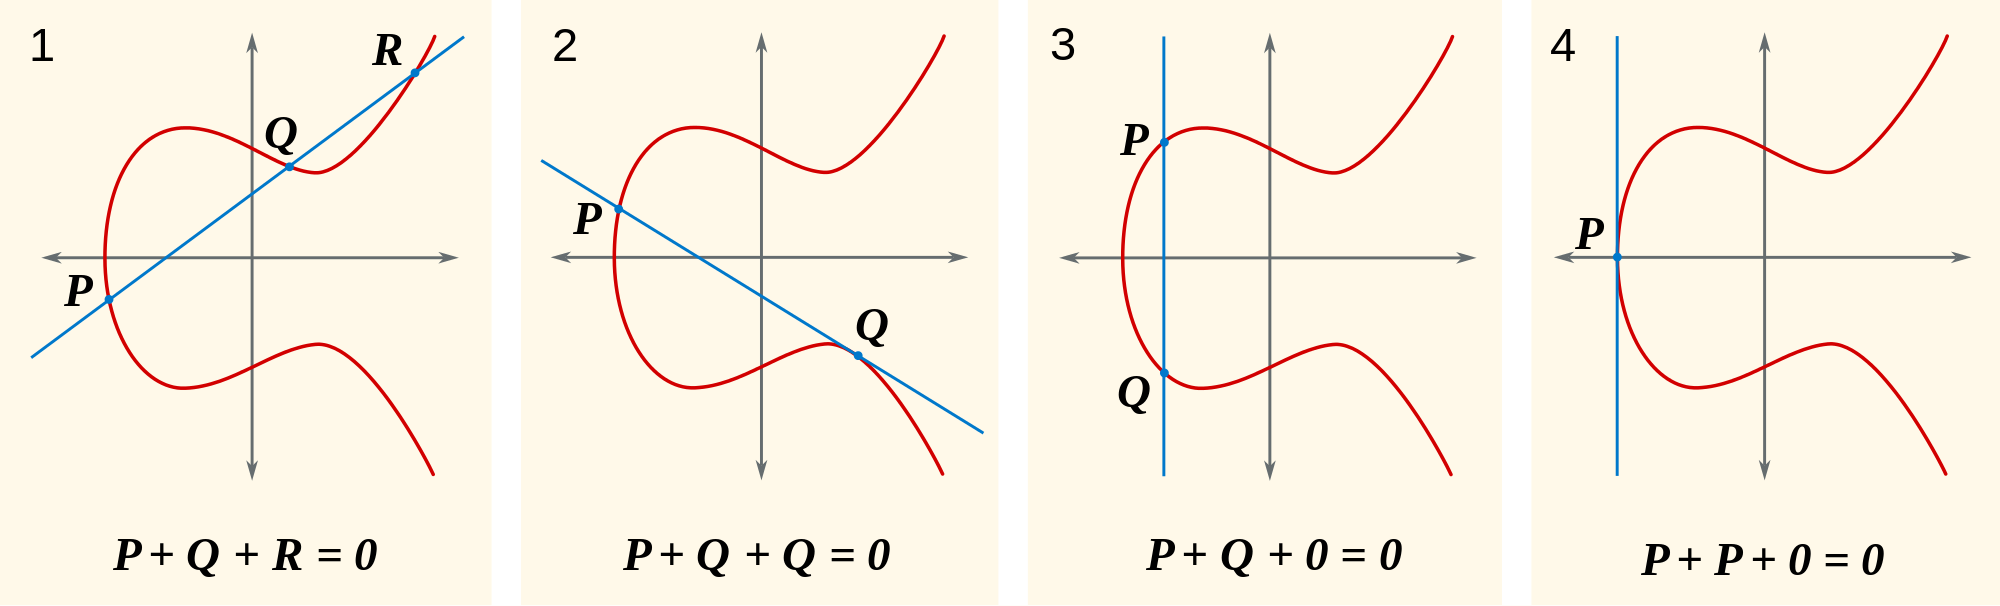
\includegraphics[scale=0.1]{ecc.png}
		
	\end{figure}
	\column{0.32\textwidth}
		\vspace{-0.2in}
		\begin{center}
			\footnotesize{
			\[kP = Q\]
			Given $P$ and $Q$, solve for $k$.}
		\end{center}
\end{columns}	
	
\begin{columns}
	\column{0.5\textwidth}
	\begin{figure}
		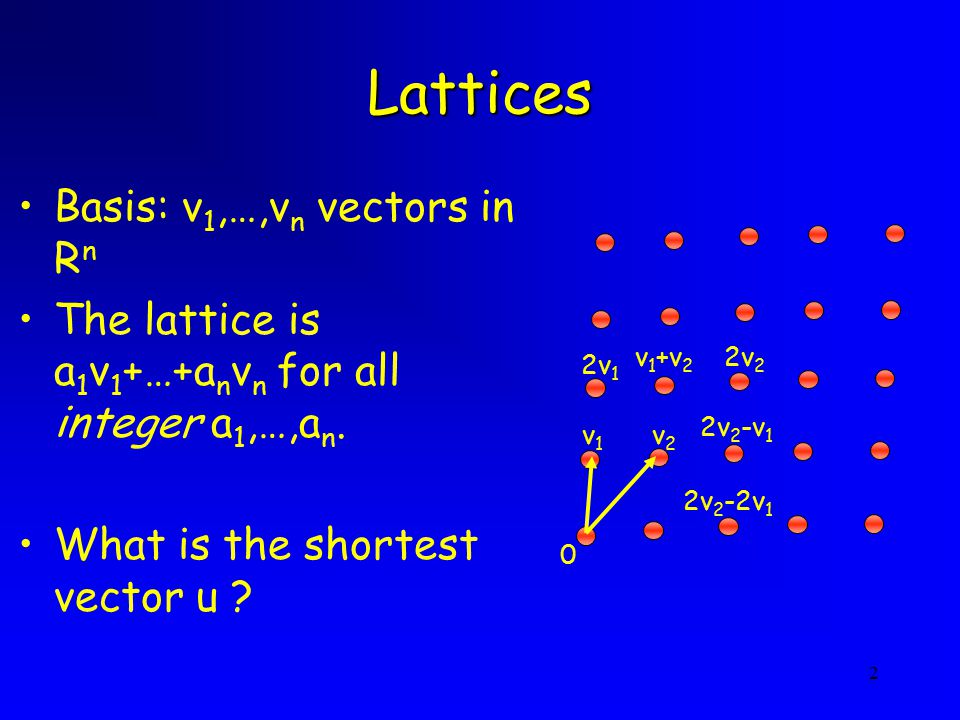
\includegraphics[scale=0.15]{lattice_crypto.jpg}
		\caption{\textbf{Lattice cryptography}}
	\end{figure}
	\column{0.5\textwidth}
	\begin{figure}
		\textbf{RSA} \\
		Let $p$ and $q$ be two distinct large primes \\
		Let $n = pq$ \\
		Given $n$, find $p$ and $q$
		
	\end{figure}
\end{columns}

\end{frame}
%***************************


%***************************
\section{Recurse Center}
\frame{\tableofcontents[currentsection]}

\begin{frame}
\frametitle{Recurse Center}

\begin{center}
	
\includegraphics[width=0.3\textwidth]{recurse_center.png}
\end{center}

\begin{center}
``The Recurse Center is a free, self-directed, educational retreat for people who want to get better at programming, whether they've been coding for three decades or three months." \\


- Recurse Center landing page
\end{center}

\end{frame}

%***************************

\begin{frame}

\frametitle{Arabic programming language}
\begin{center}

\begin{columns}
	\column{0.4\textwidth}
		\begin{figure}
			\centering{Fibbonaci sequence \\ source code \\}
			\vspace{0.1in}
			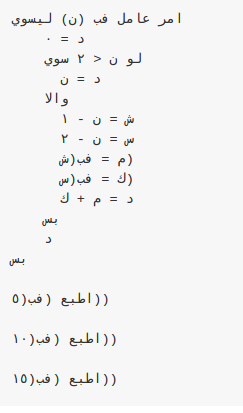
\includegraphics[scale=0.43]{ahmazing.png}
		\end{figure}
	\column{0.4\textwidth}
		\begin{figure}
			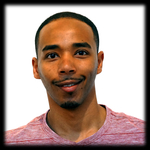
\includegraphics[scale=0.009]{ahmed.jpg}
			\caption{Ahmed Abdalla}
		\end{figure}
\end{columns}


\end{center}
\end{frame}

%***************************

\begin{frame}

\frametitle{Markov Chain Twitterbots}

\begin{columns}
	\column{0.25\textwidth}
		\begin{figure}
			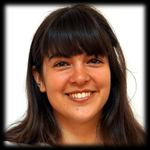
\includegraphics[scale=0.008]{sam.jpg}
			\caption{Samantha Goldstein}
		\end{figure}
	\column{0.65\textwidth}		
		\begin{figure}
			\centering{LeBron James Joyce Twitterbot}
			\vspace{0.2in}
			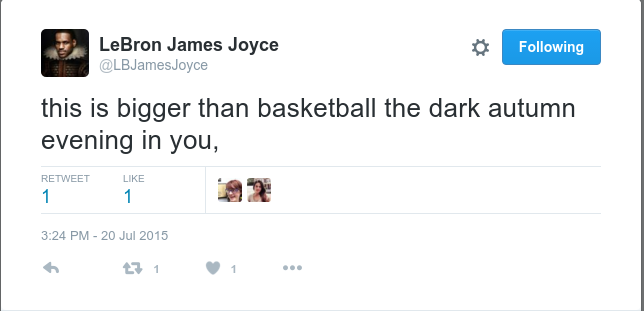
\includegraphics[scale=0.35]{ljj.png}
		\end{figure}
	
\end{columns}

\end{frame}
%***************************

\begin{frame}
\frametitle{Markov Chain Twitterbots}

\vspace{0.2in}

``You have to be able to accept failure to get better." - LeBron James

\pause

\begin{figure}
	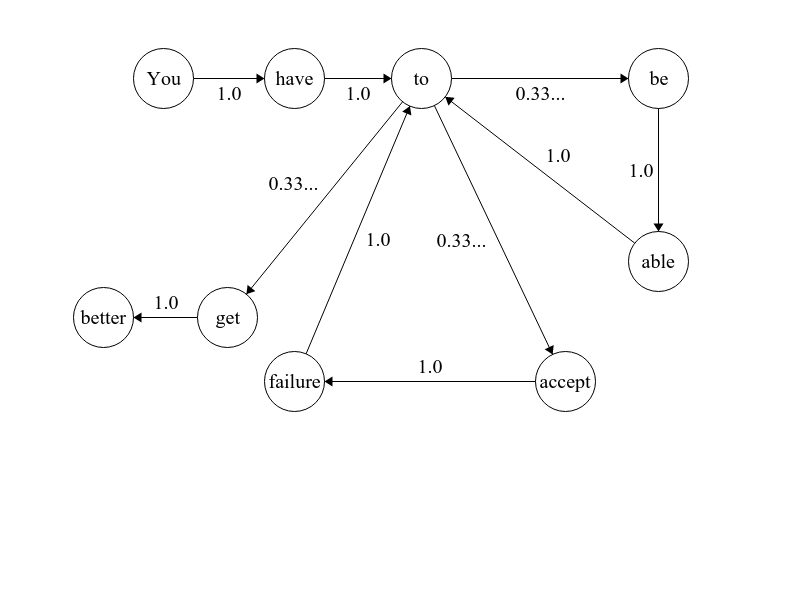
\includegraphics[scale=0.4]{lebron_graph.png}
\end{figure}

\end{frame}
%***************************
\begin{frame}
\frametitle{Markov Chain Twitterbots}
\vspace{0.2in}

``You have to be able to accept failure to get better." - LeBron James

\[ M_{i,j} = P(\text{word}_j \; | \; \text{word}_i) \]
\[
\kbordermatrix{
		& You & have & to & be & able & accept & failure & get & better \\
		You & 0 & 1 & 0 & 0 & 0 & 0 & 0 & 0 & 0 \\
		have & 0 & 0 & 1 & 0 & 0 & 0 & 0 & 0 & 0 \\
		to & 0 & 0 & 0 & 0.\overline{3} & 0 & 0.\overline{3} & 0 & 0.\overline{3} & 0 \\
		be & 0 & 0 & 0 & 0 & 1 & 0 & 0 & 0 & 0 \\
		able & 0 & 0 & 1 & 0 & 0 & 0 & 0 & 0 & 0 \\
		accept & 0 & 0 & 0 & 0 & 0 & 0 & 1 & 0 & 0 \\
		failure & 0 & 0 & 1 & 0 & 0 & 0 & 0 & 0 & 0 \\
		get & 0 & 0 & 0 & 0 &0 & 0 & 0 & 0 & 1 \\
		better & 0 & 0 & 0 & 0 &0 & 0 & 0 & 0 & 0 \\
 	}
\]


\end{frame}

%***************************

\begin{frame}
\frametitle{Markov Chain Twitterbots}
\footnotesize
\arraycolsep=3pt
\medmuskip = 1mu % default: 4mu plus 2mu minus 4mu

	\[ 
	\kbordermatrix{
		& &  & to & & & & & & \\
		& 0 & 0 & 1 & 0 & 0 & 0 & 0 & 0 & 0 \\}
	\kbordermatrix{
		& You & have & to & be & able & accept & failure & get & better \\
		 & 0 & 1 & 0 & 0 & 0 & 0 & 0 & 0 & 0 \\
		 & 0 & 0 & 1 & 0 & 0 & 0 & 0 & 0 & 0 \\
		 & 0 & 0 & 0 & 0.\overline{3} & 0 & 0.\overline{3} & 0 & 0.\overline{3} & 0 \\
		 & 0 & 0 & 0 & 0 & 1 & 0 & 0 & 0 & 0 \\
		 & 0 & 0 & 1 & 0 & 0 & 0 & 0 & 0 & 0 \\
		 & 0 & 0 & 0 & 0 & 0 & 0 & 1 & 0 & 0 \\
		 & 0 & 0 & 1 & 0 & 0 & 0 & 0 & 0 & 0 \\
		 & 0 & 0 & 0 & 0 &0 & 0 & 0 & 0 & 1 \\
		 & 0 & 0 & 0 & 0 &0 & 0 & 0 & 0 & 0 \\
 	} \]
 	\[
 	= \kbordermatrix{
 		& & & & be & & accept& & get & \\
 		& 0 & 0 & 0 & 0.\overline{3} & 0 & 0.\overline{3} & & 0.\overline{3} & 0 \\
 	}
\]
\end{frame}

%***************************

\begin{frame}
\frametitle{Recurse Center}

\centering{\huge The Social Rules }
\begin{center}
	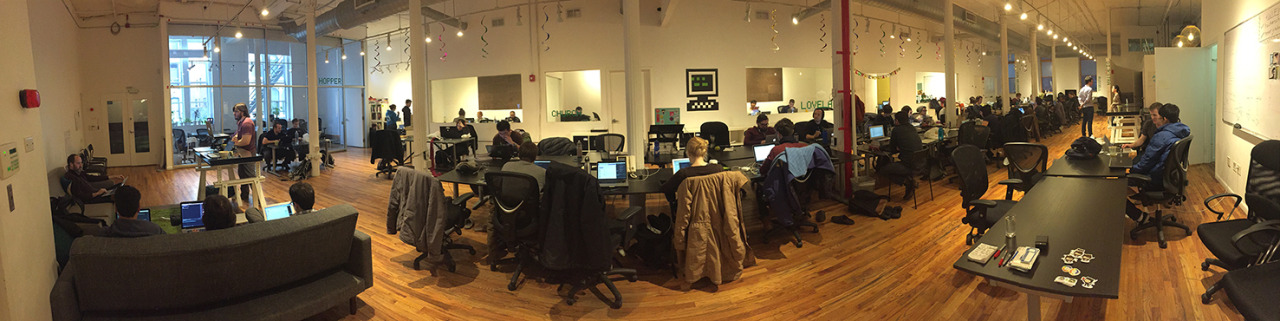
\includegraphics[width=\textwidth]{recursers}
\end{center}

\begin{columns}[c]
	\column{0.1\textwidth}
	\column{0.5\textwidth}
		\begin{itemize}
			\item No feigning surprise
			\item No well-actually's
		\end{itemize}
	\column{0.5\textwidth}
		\begin{itemize}
			\item No back-seat driving
			\item No subtle -isms
		\end{itemize}
	\column{0.1\textwidth}
\end{columns}

\end{frame}



%***************************
\section{EMC}
\frame{\tableofcontents[currentsection]}

\begin{frame}
\frametitle{Software Engineering}
    \begin{figure}
        \centering
        \begin{minipage}{.5\textwidth}
            \centering
            
\includegraphics[width=.8\linewidth]{EMC-Corporation.jpg}

        \end{minipage}%
        \pause
        \begin{minipage}{.5\textwidth}
            \centering
            
\includegraphics[width=.7\linewidth]{Dell_EMC.png}
           
        \end{minipage}
        
    \end{figure}
    
\centering 
Soon to be.....

\end{frame}

%***************************

\begin{frame}
\frametitle{Software Engineering}
\begin{figure}
	\begin{center}
		
\includegraphics[scale=0.50]{xio_logo} 
	\end{center}
\end{figure}

\begin{columns}
	\column{0.3\textwidth}
		\vspace{-0.2in}
		\begin{figure}
			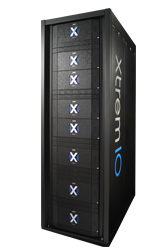
\includegraphics[scale=0.5]{xio.png}
			\caption{Cluster}
		\end{figure} 
	\column{0.4\textwidth}
		\pause
		\begin{figure}
		 	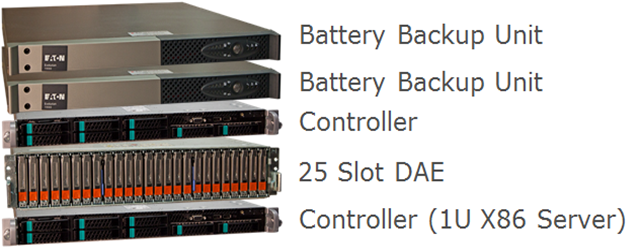
\includegraphics[scale=0.25]{xbrick.png}
		 	\caption{Xbrick}
		\end{figure}
	\column{0.3\textwidth}
		\pause
		\begin{figure}
			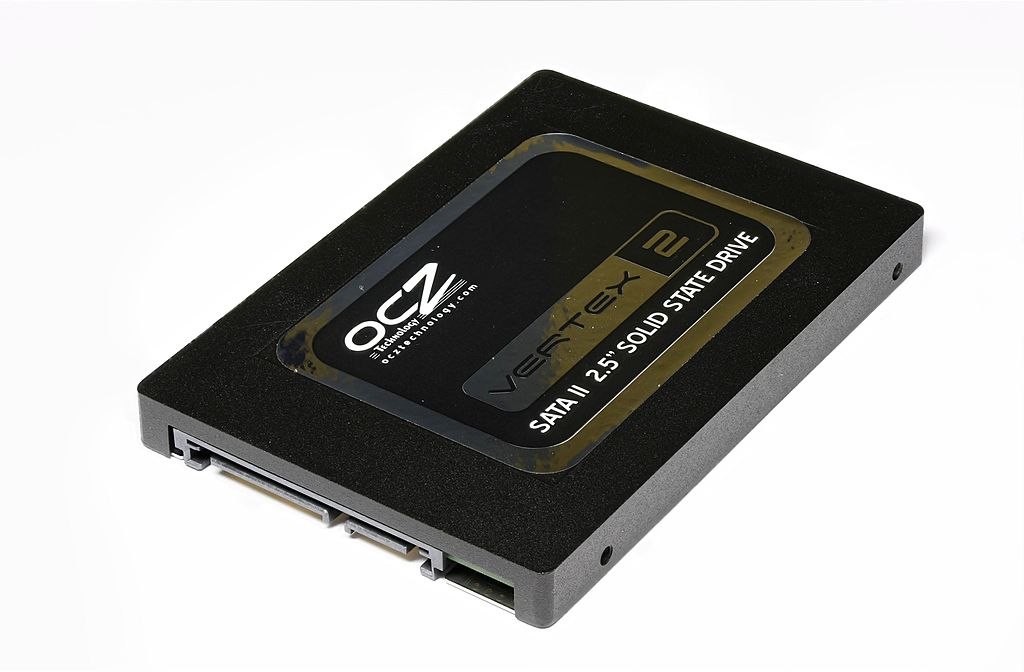
\includegraphics[scale=0.10]{ssd.jpg}
			\caption{Solid-state drive (SSD)}
		\end{figure}
\end{columns}
\end{frame}

%***************************

\begin{frame}
\frametitle{Word Problem!}
An engineer at EZIO is trying to design a new storage device
\vspace{0.2in}
	\begin{itemize}
		\item RealCompany SSDs have an annual failure rate of 9 in 1000
		\pause
		\vspace{0.1in}
		\item The engineer wants each EZbrick to contain 25 drives
		\pause
		\vspace{0.1in}
		\item The lifetime of an EZbrick is about 5 years
		\pause
		\vspace{0.1in} 
		\item The engineer expects to sell 100 EZbricks as soon as they become available
	\end{itemize}
\pause
\vspace{0.2in}
What is the probability of a drive failure in any of those 100 EZbricks over the span of their lifetime?

	
\end{frame}

%***************************
\begin{frame}
\frametitle{Word Problem!}

\begin{center}
	\begin{tabular}{ | c | c | }
		\hline Annual failure rate & 0.009 \\
		\hline Drives per EZbrick & 25 \\
		\hline EZbrick lifetime & 5 years \\
		\hline EZbricks & 100 \\
		\hline 	
	\end{tabular}
\end{center}

\pause
\[ P(\text{failure in single EZbrick after 1 year} ) = 1 - (1 - 0.009)^{25} \approx 0.20\]
\pause
\[P(\text{failure in single EZbrick after lifetime} ) = 1 - (1 - 0.20)^5 \approx 0.67\]
\pause
\[P(\text{failure in 100 EZbricks after lifetime} ) = 1 - (1 -.67)^{100} \approx .99 \]
\pause
\begin{center}
This is going to happen
\end{center}
\end{frame}
%***************************

\begin{frame}
\frametitle{RAID}

	\begin{center}
		Redundant Array of Inexpensive/Independent Disks
		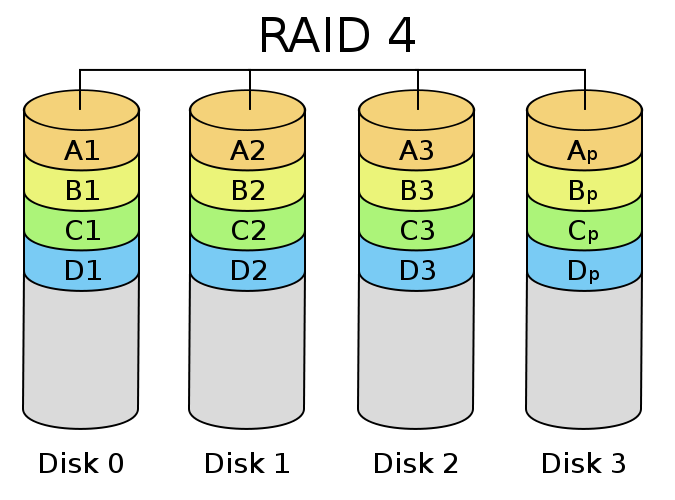
\includegraphics[width=0.5\linewidth]{raid4}	
	\end{center}
\end{frame}

%***************************

\begin{frame}
\frametitle{RAID}

\begin{columns}
	\column{0.3\textwidth}
		\begin{center}
			\vspace{-1in}
			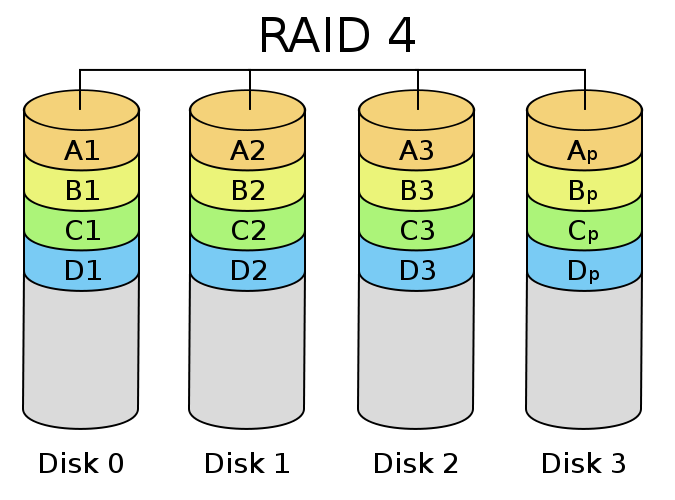
\includegraphics[scale=0.15]{raid4}	
		\end{center}
	\column{0.7\textwidth}
		\begin{center}
		Let's say each ``chunk" of a disk stores 1 bit, either a 0 or a 1
		\pause
		\[A_p \equiv A1 + A2 + A3 \pmod 2\]
		\pause \[ A1 = 1, \; \; A2 = 1, \; \; A3 = 0, \;\;  A_p = \pause 0\]
		\pause \[ A1 = 0, \; \; A2 = 1 \;\; A3 = 0, \;\; A_p = \pause 1\]
		\pause \[ A1 = 1, \;\; A2 = 1 \;\; A3 = 1, \;\; A_p = \pause 1\]
		\end{center}
\end{columns}

\end{frame}

%***************************

\begin{frame}
\frametitle{RAID}

\begin{columns}
	\column{0.3\textwidth}
		\begin{center}
			\vspace{-1in}
			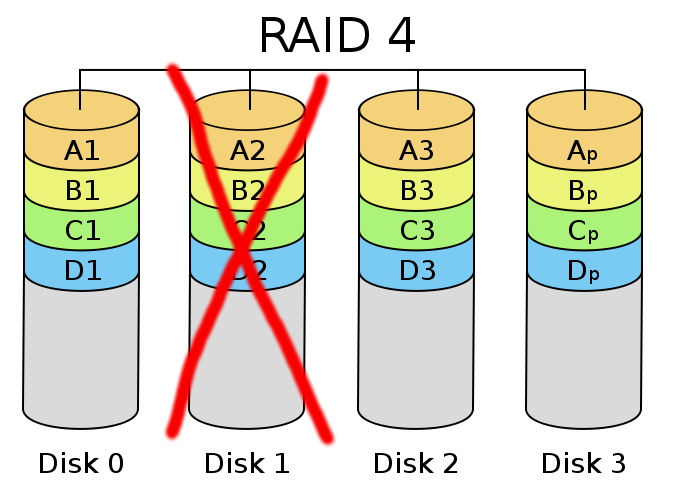
\includegraphics[scale=0.15]{disk1}	
		\end{center}
	\column{0.7\textwidth}
		\begin{center}
			So when a drive goes down, the data that was stored in it can be recovered! 
		
			\[A1 = 1, \; \; A2 = ???, \; \; A3 = 1, \;\; A_p =  0\]
		    \pause \[ A_p \equiv A1 + A2 + A3 \pmod 2 \]
		    \vspace*{-\baselineskip}\pause\[ 0 \equiv 1 + x + 1 \pmod2 \]
		    \vspace*{-\baselineskip}\pause\[ \; 0 \equiv 2 + x \pmod 2 \quad \quad \]
		   \vspace*{-\baselineskip} \pause \[ 0 \equiv x \pmod 2 \quad \quad \quad \;\; \]
		\end{center}
\end{columns}
 
\end{frame}

%***************************
\begin{frame}
\frametitle{Word Problem II!}

	\begin{center}
		We've dealt with a single disk failure, but what about 2 disk failures?!?! At the SAME TIME?!?!
	\end{center}
	
\end{frame}
%***************************

%***************************
\begin{frame}
\frametitle{Word Problem II!}
	
	\begin{center}
		What counts as ``the same time?" \\
		How long does it take for a disk to fail and then be recovered? \\
		
		\pause 
		\vspace{0.2in}
		Let's play it safe and say a whole day. 
	\end{center}
	
\end{frame}
%***************************

\begin{frame}
\frametitle{Word Problem II!}

\begin{center}
	\begin{tabular}{ | c | c | }
		\hline Annual failure rate & 0.009 \\
		\hline Drives per EZbrick & 25 \\
		\hline EZbrick lifetime & 5 years \\
		\hline EZbricks & 100 \\
		\hline 	
	\end{tabular}
\end{center}

\begin{center}
	We have annual failure rate... but we need daily failure rate.

\pause

\[ P(\text{disk failure in N years}) = 1 - (1 - 0.009)^N \]
\vspace*{-\baselineskip} \pause  \[ = 1 - (1 - 0.009)^{N*(365/365)} \]
\vspace*{-\baselineskip} \pause \[ = 1 - (1 - 0.009)^{(1/365)^{N*365}} \]
\vspace*{-\baselineskip} \pause \[ = 1 - 0.991^{(1/365)^{N*365}}\]
\vspace*{-\baselineskip} \pause \[ \approx 1 - (0.9999752)^{N*365}\]
\vspace*{-\baselineskip} \pause \[ P(\text{disk failure in N days}) \approx 1 - (1 - 0.0000248) ^N \]

\end{center}

	
\end{frame}
%***************************

\begin{frame}
\frametitle{Word Problem II!}

\begin{center}
	\begin{tabular}{ | c | c | }
		\hline Annual failure rate & 0.009 \\
		\hline Drives per EZbrick & 25 \\
		\hline EZbrick lifetime & 5 years \\
		\hline EZbricks & 100 \\
		\hline Daily failure rate & 0.0000248 \\
		\hline
	\end{tabular}
\end{center}

\begin{center}
For a single day and 1 EZbrick...
	\[P(>\text{1 disk failure}) = P( \geq \text{1 disk failure}) - P(\text{exactly 1 disk failure})  \]
\vspace*{-\baselineskip} \pause	\[ = (1 - (1 - 0.0000248)^{25}) - {25\choose 1}(0.0000248)(1 - 0.0000248)^{24}\]
\vspace*{-0.5\baselineskip} \pause\[0.000619816 - 0.000619631 \approx 1.85\times10^{-7} \]

\end{center}
	
\end{frame}

%**********************

\begin{frame}
\frametitle{Word Problem II!}

\begin{center}
	\begin{tabular}{ | c | c | }
		\hline Annual failure rate & 0.009 \\
		\hline Drives per EZbrick & 25 \\
		\hline EZbrick lifetime & 5 years \\
		\hline EZbricks & 100 \\
		\hline Daily failure rate & 0.0000248 \\
		\hline
	\end{tabular}
\end{center}

\begin{center}
\[P( >1\text{ failure in 1 EZbrick over 1 day}) \approx 1.85 \times 10^{-7}\]
\vspace*{-0.5\baselineskip} \pause \[P( >1\text{ failure in 1 EZbrick over lifetime}) = 1 - (1 - 1.85\times 10^{-7})^{365*5} \]
\[ \approx 0.000338\]
\vspace*{-0.5\baselineskip} \pause\[ P( > 1 \text{ failure in 100 EZbricks over lifetime}) = 1 - (1 - 0.000338)^{100} \]
\[\approx 0.0332 \]
\end{center}

\end{frame}

%**********************
\section{Wrap it Up}

\frame{\tableofcontents[currentsection]}

\begin{frame}
\frametitle{Math helps us answer questions...}

\begin{center}
	\vspace{-0.1in}
	\begin{columns}
		\column{0.4\textwidth}
			...about beautiful things 
		\column{0.2\textwidth}
			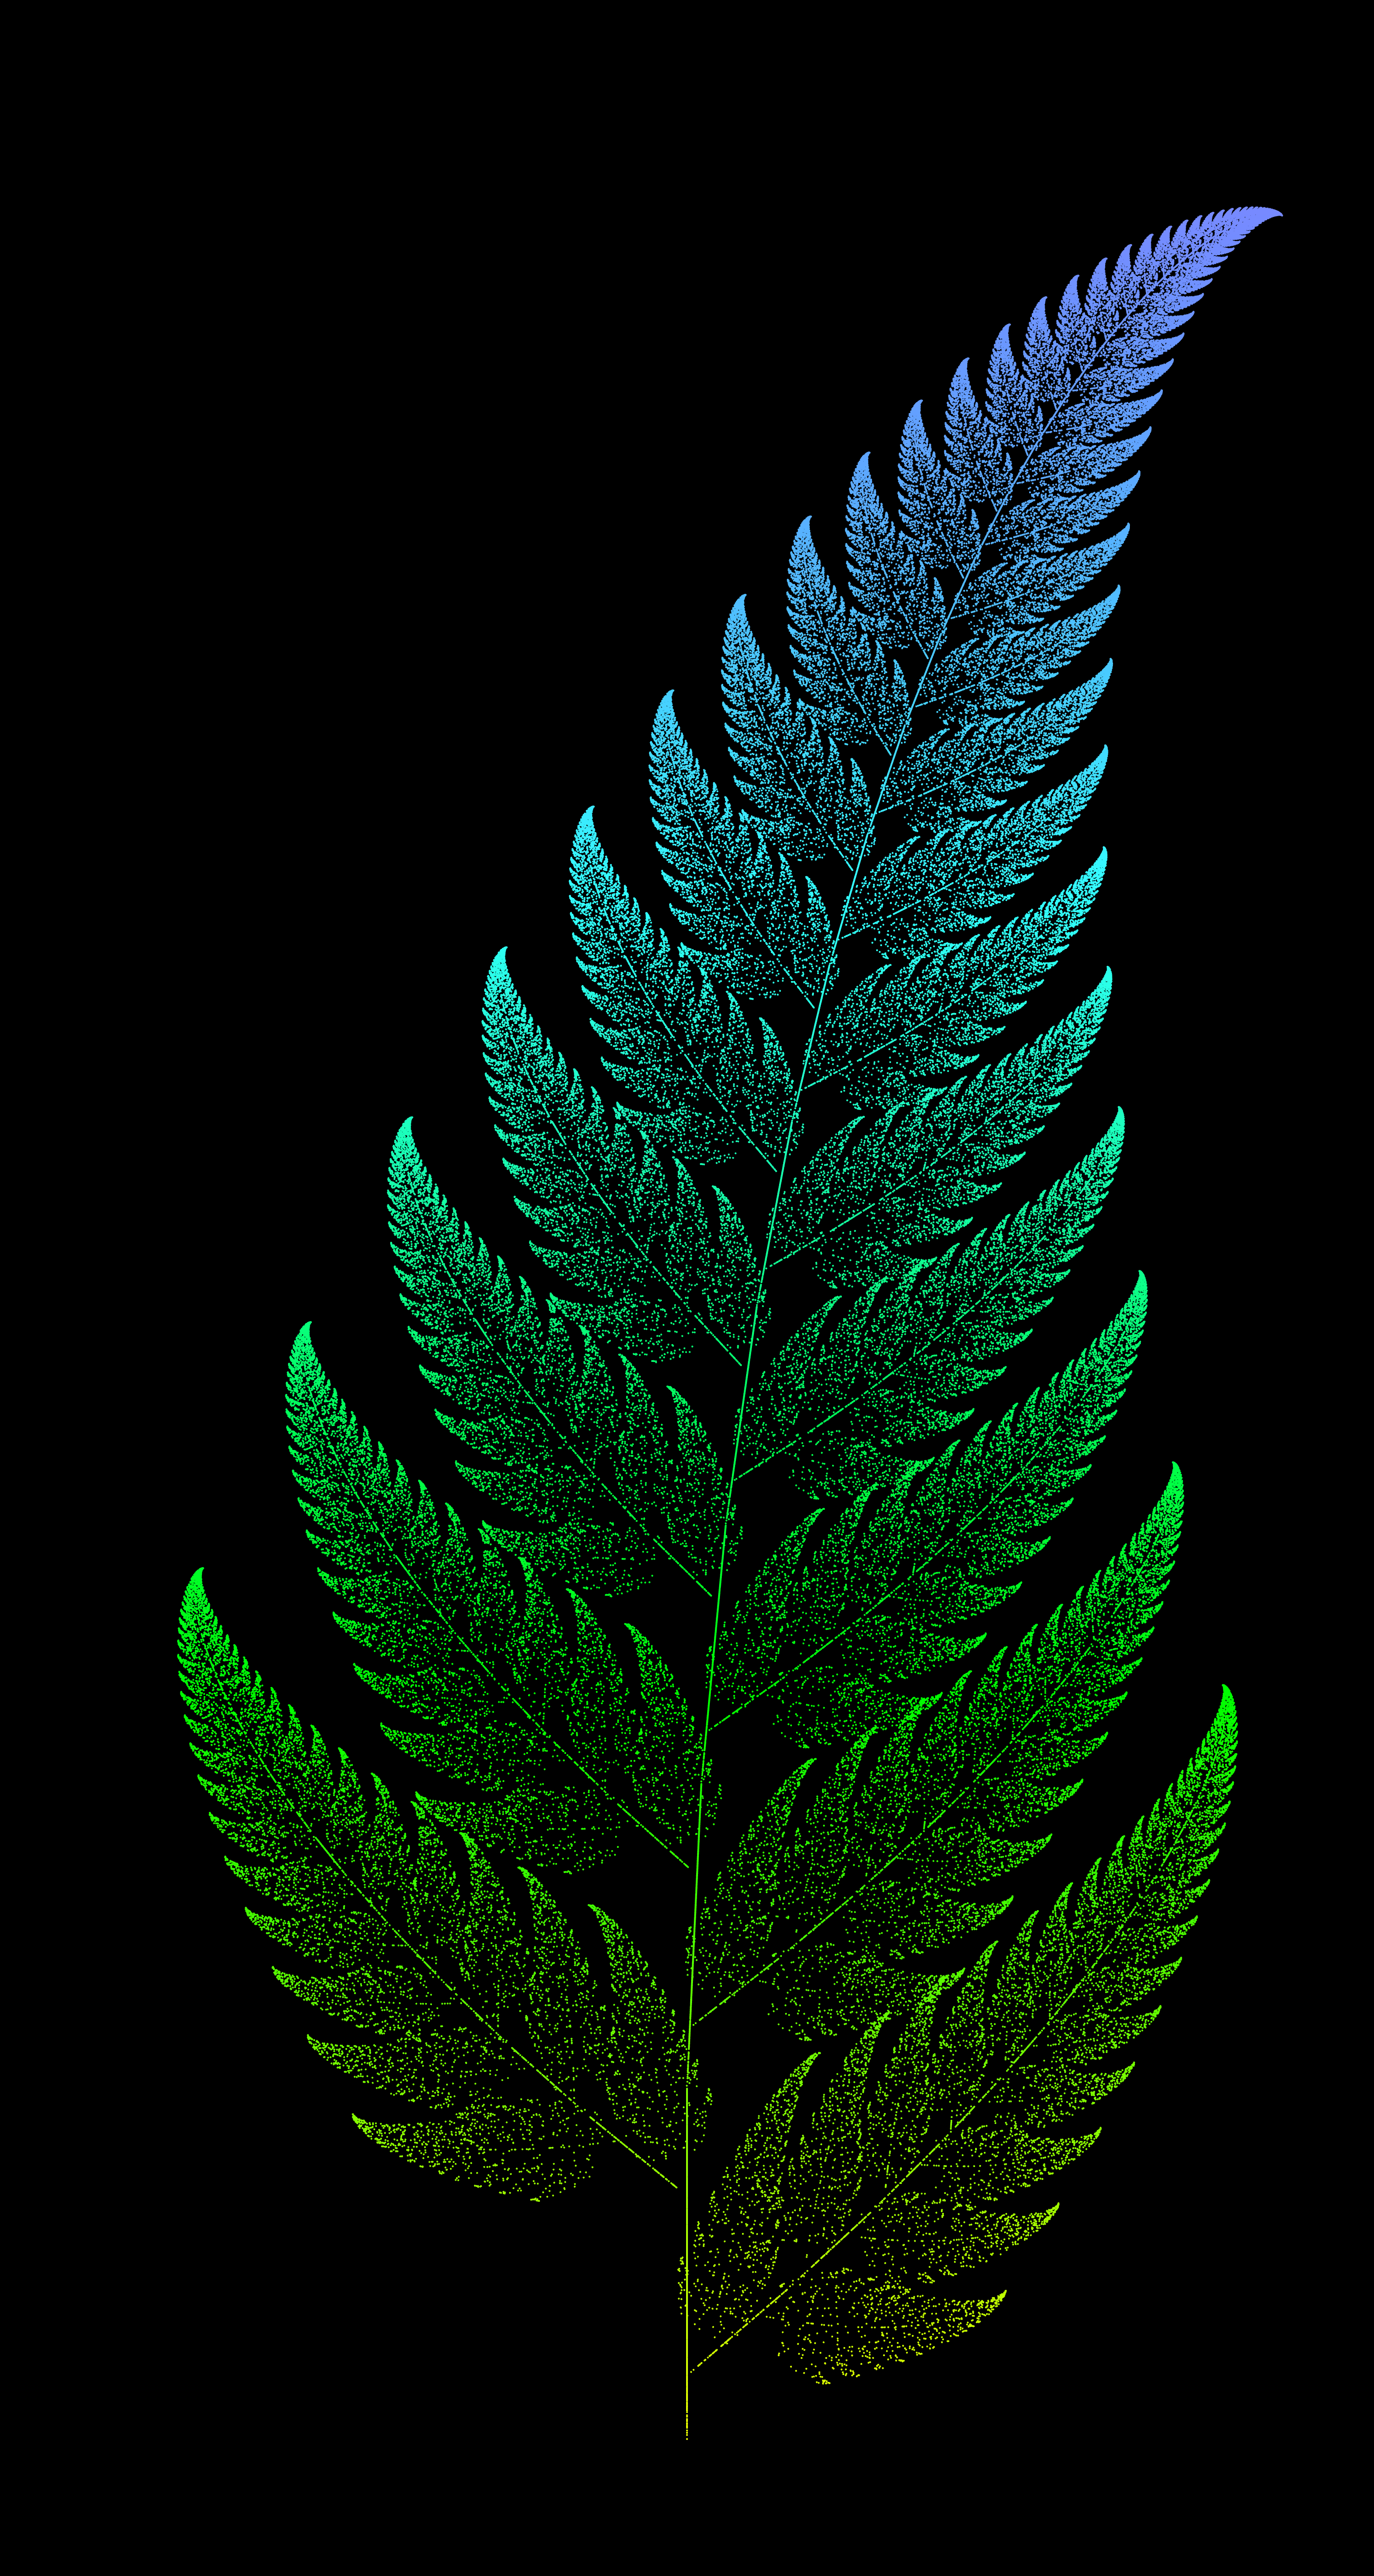
\includegraphics[scale=0.017]{fern.png}
		\column{0.2\textwidth}
	\end{columns}
	\vspace{-0.3in}
	\begin{columns}
		%\column{0.1\textwidth}
		\column{0.3\textwidth}
			\vspace{-0.4in} \includegraphics[scale=0.45]{lebron.jpg} 
		\column{0.6\textwidth}
			...about silly things
	\end{columns}
	\begin{columns}
		\column{0.3\textwidth}
		\column{0.2\textwidth}
			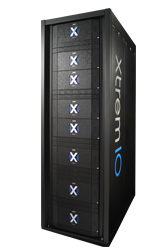
\includegraphics[scale=0.3]{xio.png}
		\column{0.5\textwidth}
			...about business-critical things
	\end{columns}
\end{center}

\end{frame}

%**********************

\begin{frame}
\frametitle{You give us the confidence to ask questions of our own}

\begin{center}
\pause
\huge{\textbf{Thank you!}}

\pause

\vspace{0.3in}
\small{
Email: optimistindustries@gmail.com \\
Web: optimistindustries.com \\
Twitter: @optimistsinc
}
\end{center}


\end{frame}


%**********************
\end{document}